\documentclass[blue]{beamer}

%In order for this file to compile correctly you must us pdfLatex to compile instead of the normal LaTeX.
% In addition to that, all figures included must be *.pdf
% To change the style of the slide show you just change the style name (example: \usepackage{beamerthemeilmenau} )
% For more styles please visit http://mike.depalatis.net/beamerthemes/
% This site shows the names of all the available styles as well as picture of each!
%\documentclass[red]{beamer} changes the color. I know red and blue work (blue is default) However, I'm not sure
% what other colors are available! Have Fun!!

% \usepackage{beamerthemeHannover}
%\usepackage{beamerthemeDresden}
%\usepackage{beamerthemeBerlin}
% \usepackage{beamerthemeIlmenau}
\setbeamertemplate{blocks}[rounded][shadow=true]
\setbeamertemplate{frametitle}
{
  \begin{centering}
    \vspace*{0.2in}
    \color{blue}
    \textbf{\insertframetitle}
    \par
  \end{centering}
}

% fancybox is included in case I want to change my slide frame or titles 
% into something more interesting
\usepackage{fancybox}
\usepackage{shadow}

\usepackage{amsmath}
% 
\newcommand{\pair}[1]{\ensuremath{\langle #1\rangle}}
\newcommand{\annd}{\ensuremath{\ \&\ }}
\newcommand{\orr}{\ensuremath{\textrm{ or }}}
\newcommand{\pow}[1]{\ensuremath{\mathcal{P}(#1)}}
\newcommand{\set}[1]{\ensuremath{\{#1\}}}
\newcommand{\midset}[2]{\ensuremath{\set{#1 \mid #2}}}
\newcommand{\arrow}{\ensuremath{\rightarrow}}
\newcommand{\id}[1]{\ensuremath{\textsf{id}_{#1}}}

\newcommand{\isa}{\ensuremath{\; {:}{:}{=} \;}}
\newcommand{\ora}{\ensuremath{\;\mid\;}}

\newcommand{\subst}[3]{\ensuremath{{#1}\boldsymbol{[}#2\boldsymbol{/}#3\boldsymbol{]}}} 

% Miscellaneous

\newcommand{\defined}{\ensuremath{\quad \triangleq \quad}}
\newcommand{\defn}{\ensuremath{\stackrel{\mathrm{def}}{=}}}

\newcommand{\key}[1]{\textbf{#1}}



% Syntactic sets
\newcommand{\PName}{\ensuremath{\textbf{PName}}}
\newcommand{\PExp}{\ensuremath{\textbf{Princ}}}
\newcommand{\PropVar}{\ensuremath{\textbf{PropVar}}}
\newcommand{\LExp}{\ensuremath{\textbf{Form}}}
%\newcommand{\privs}{\ensuremath{\mathit{privs}}}
%\newcommand{\Targ}{\ensuremath{\mathcal{T}}}

\newcommand{\says}{\ensuremath{\text{\footnotesize \textsf{ says }}}}
\newcommand{\controls}{\ensuremath{\text{\footnotesize \textsf{ controls }}}}
%\newcommand{\controls}{\ensuremath{\textsf{\footnotesize controls }}}
%\newcommand{\serves}{\ensuremath{\textsf{ serves }}}
%\newcommand{\speaksfor}{\ensuremath{\textsf{ speaks\_for }}}
\newcommand{\speaksfor}{\ensuremath{\Rightarrow}}

\newcommand{\serves}[1]{\ensuremath{\ \mathsf{serves}_{#1}\ }}
\newcommand{\quoting}{\ensuremath{\,|\,}}
\newcommand{\with}{\ensuremath{\,\&\,}}
\newcommand{\for}[1]{\ensuremath{\ \mathsf{for}_{#1}\ }}

%\newcommand{\name}[1]{\textit{#1}}
\newcommand{\act}[1]{\ensuremath{\langle #1\rangle}}



\newcommand{\krip}[1]{\ensuremath{\langle {#1} \rangle}}

\newcommand{\E}[1]{\ensuremath{\mathcal{E}_{\mathcal{M}}[\![#1]\!]}}
\newcommand{\Em}[2]{\ensuremath{\mathcal{E}_{#2}[\![#1]\!]}}


\newcommand{\rulespace}{\vspace*{1.8em}}
\newcommand{\infrule}[2]
   {\ensuremath{{\textstyle #1}\over{\textstyle #2}}}

%\newcommand{\deriv}{\ensuremath{\vdash}}

% inference rule with name

%\newcommand{\irule}[3]
%   {\ensuremath{\mathrm{#3}\; {{\textstyle {#1} }\over {\textstyle{#2}}}}}

\newcommand{\infname}[1]{\textit{#1}}

\newcommand{\irule}[3]
    {\ensuremath{\infname{#3}\quad {\displaystyle \frac{#1}{#2}}}}
% if then else

\newcommand{\ite}[3]
   {\ensuremath{#1 \rightarrow #2 \mid #3}}

\renewcommand{\implies}{\supset}

\newcommand{\name}[1]{\ensuremath{\textit{#1}}}

\newcommand{\reps}[3]{\ensuremath{{#1} \text{\footnotesize \textsf{
          reps }}{#2}{\text{\footnotesize \textsf{ on }}}{#3}}}
\newcommand{\rp}[2]{\ensuremath{{#1} {\text{\footnotesize \textsf{
          reps }}}{#2}{\text{\footnotesize \textsf{ on }}}}}

% \usepackage[dvipsnames,usenames]{color}
\newcommand{\redtext}[1]{\textcolor{red}{#1}}
\newcommand{\bluetext}[1]{\textcolor{blue}{#1}}

% \newif\ifpdf
%   \usepackage[pdftex]{graphicx}
%   \pdfcompresslevel=9
%   \pdfpagewidth=11truein %297truemm % your milage may vary....
%   \pdfpageheight=8.5truein %210truemm
%   \pdfhorigin=1truein     % default value(?), but doesn't work without
%   \pdfvorigin=1truein     % default value(?), but doesn't work without
% \else
%   \usepackage{graphicx}
% \fi
\usebackgroundtemplate{

\includegraphics[width=\paperwidth,height=\paperheight]{Figures/AFRLTitle.jpg}}

\title{An Overview of the Access-Control Logic in Higher-Order Logic}
\author[]{Shiu-Kai Chin, Ph.D.}
\institute[Syracuse University/Serco North America] % (optional, but mostly needed)
{Syracuse University\\
 Department of Electrical Engineering and Computer Science\\
 Syracuse, NY 13244\\
\vspace{0.1in}
 Serco North America\\
 7900 Turin Road\\
 Rome, NY 13440}
\date{\today}



\begin{document}

\frame{\titlepage}

\setbeamertemplate{background}
{
\includegraphics[width=\paperwidth,height=\paperheight]{Figures/AFRLBackground.jpg}}

\frame{\frametitle{Motivation}
% \vspace{0.2in}
\begin{center}
  \Large{\emph{Doveryai, no proveryai}}\\
  \Large{(Trust, but verify)}\\
\end{center}
}

% \frame{\frametitle{Attitude}
%   \begin{center}
%     \Large{\emph{With willing hearts and skillful hands, the difficult
%         we do at once; the impossible takes a bit longer.}}\\
% \vspace{0.1in}
%     \footnotesize{-- Inscription on the memorial to the Seabees (U.S. Naval
%     Construction Batallions), between Memorial Bridge and Arlington
%     Cemetery}
%   \end{center}
% }

\frame{\frametitle{Orientation: Elements of Trust}
Trust has two components:
\begin{enumerate}
\item<2-> Verification
  \begin{itemize}
  \item<3-> Formal proofs using a logic with formal semantics
  \end{itemize}

\item<4-> Accountability to independent third-parties
  \begin{itemize}
  \item<5-> Auditable by independent third-parties
  \item<6-> Easily inspected, reproducible, and reusable with trusted tools
  \end{itemize}

\end{enumerate}
}

\frame{\frametitle{Why?}
  \begin{itemize}
  \item<2-> Common Criteria evaluation assurance level 7 (EAL7)
    \begin{itemize}
    \item<3-> Designs and implementations are formally verified and tested
    \end{itemize}
  \item<4-> EAL7 is applicable to the development of security TOEs
    (targets of evaluation) for application in extremely high risk
    situations and/or where the high value of the assets justifies the
    higher costs.
    \begin{itemize}
    \item<5-> Practical application of EAL7 is currently limited to
      TOEs with tightly focused security functionality that is
      amenable to extensive formal analysis.
  \end{itemize}
\item<6-> Must address formal description, verification, and tools
  \begin{itemize}
  \item<7-> This is a limiting factor to trustworthiness
  \end{itemize}

    \end{itemize}

}

\begin{frame}
  \frametitle{Purpose}
  Show how to provide assurance to engineers designing access-control
  mechanisms such that:
  \begin{itemize}
  \item<2-> Trust assumptions, jurisdiction,  delegation, and policies are
    explicitly formulated
  \item<3-> Behavior of mechanisms and policies are theorems provable in an
    access-control logic
  \item<4-> Design verification is supported by automated tools
  \item<5-> Design verification is auditable and reproducible by
    independent third parties
  \end{itemize}

\end{frame}

\begin{frame}
  \frametitle{Roadmap}
  \begin{enumerate}
  \item<2-> What we're aiming for
    \begin{itemize}
    \item<3-> Common capabilities for design engineers, verification
      engineers, and certifiers
    \end{itemize}

  \item<4-> Components
    \begin{itemize}
    \item<5-> Access-control logic (pencil and paper) based on Kripke semantics
    \item<5-> Inference rules used by specifiers, designers, and verifiers
    \item<5-> Higher-Order Logic (HOL) proof checker (theorem prover)
    \end{itemize}
  \item<6-> Rigorous connections among components that provide a sound
    foundation for trustworthiness
    \begin{itemize}
    \item<7-> Establishing and preserving logical consistency
    \end{itemize}
  \item<8-> Applications and examples

  \end{enumerate}
\end{frame}
\begin{frame}
  \frametitle{1. What We're Aiming For}
  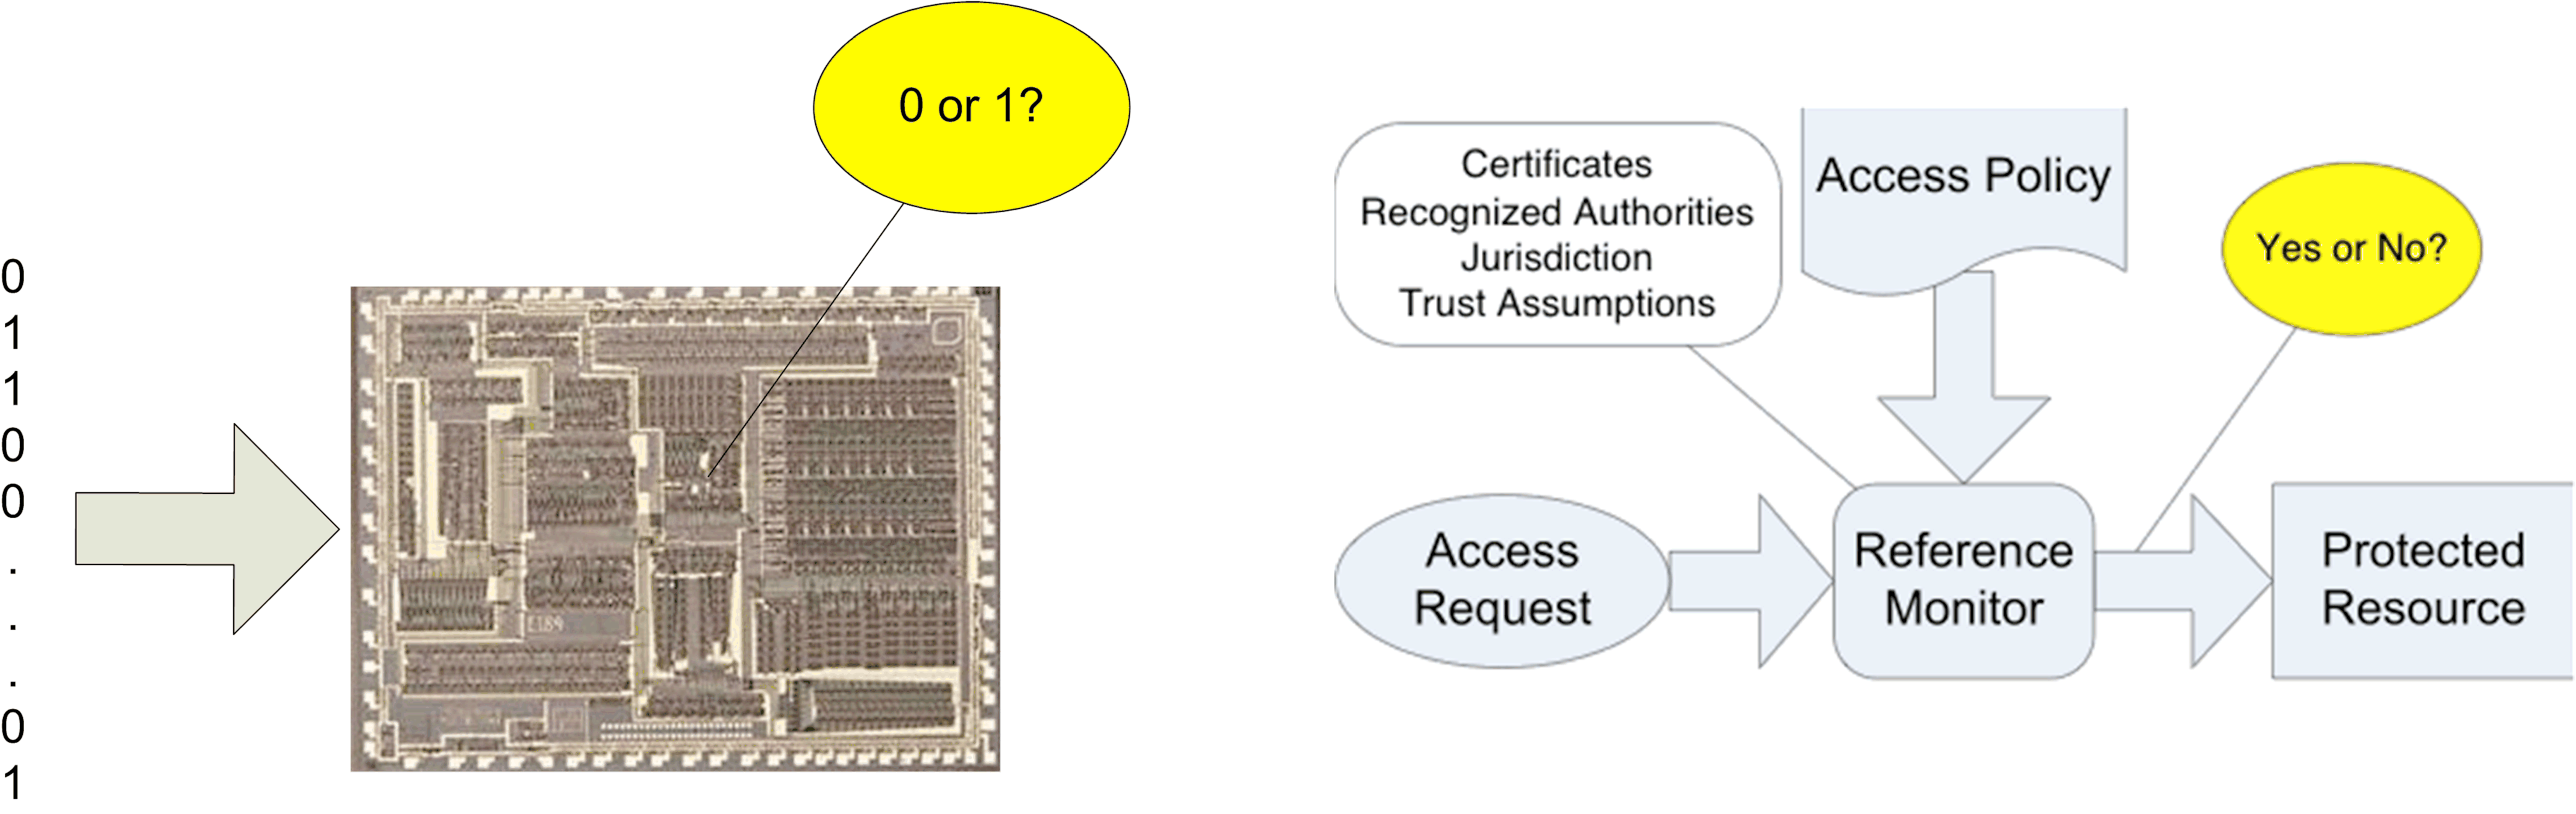
\includegraphics[width=4in]{Figures/Expectations}
  \begin{itemize}
  \item<2-> Expectations of chip designers
    \begin{itemize}
    \item<3-> At any location in the chip: when given primary inputs
      and register state, provide a formal derivation of whether the
      output is a 0 or 1.
    \end{itemize}
  \item<4-> Expectations of security engineers
    \begin{itemize}
    \item<5-> For any protected resource: when given a request,
      certificates, recognized authorties, jurisdictions, trust
      assumptions, and access policies, provide a formal derivation of
      whether or not the request is granted.
    \end{itemize}
  \end{itemize}
\end{frame}

\frame{\frametitle{What are we talking about?}
  \begin{center}
    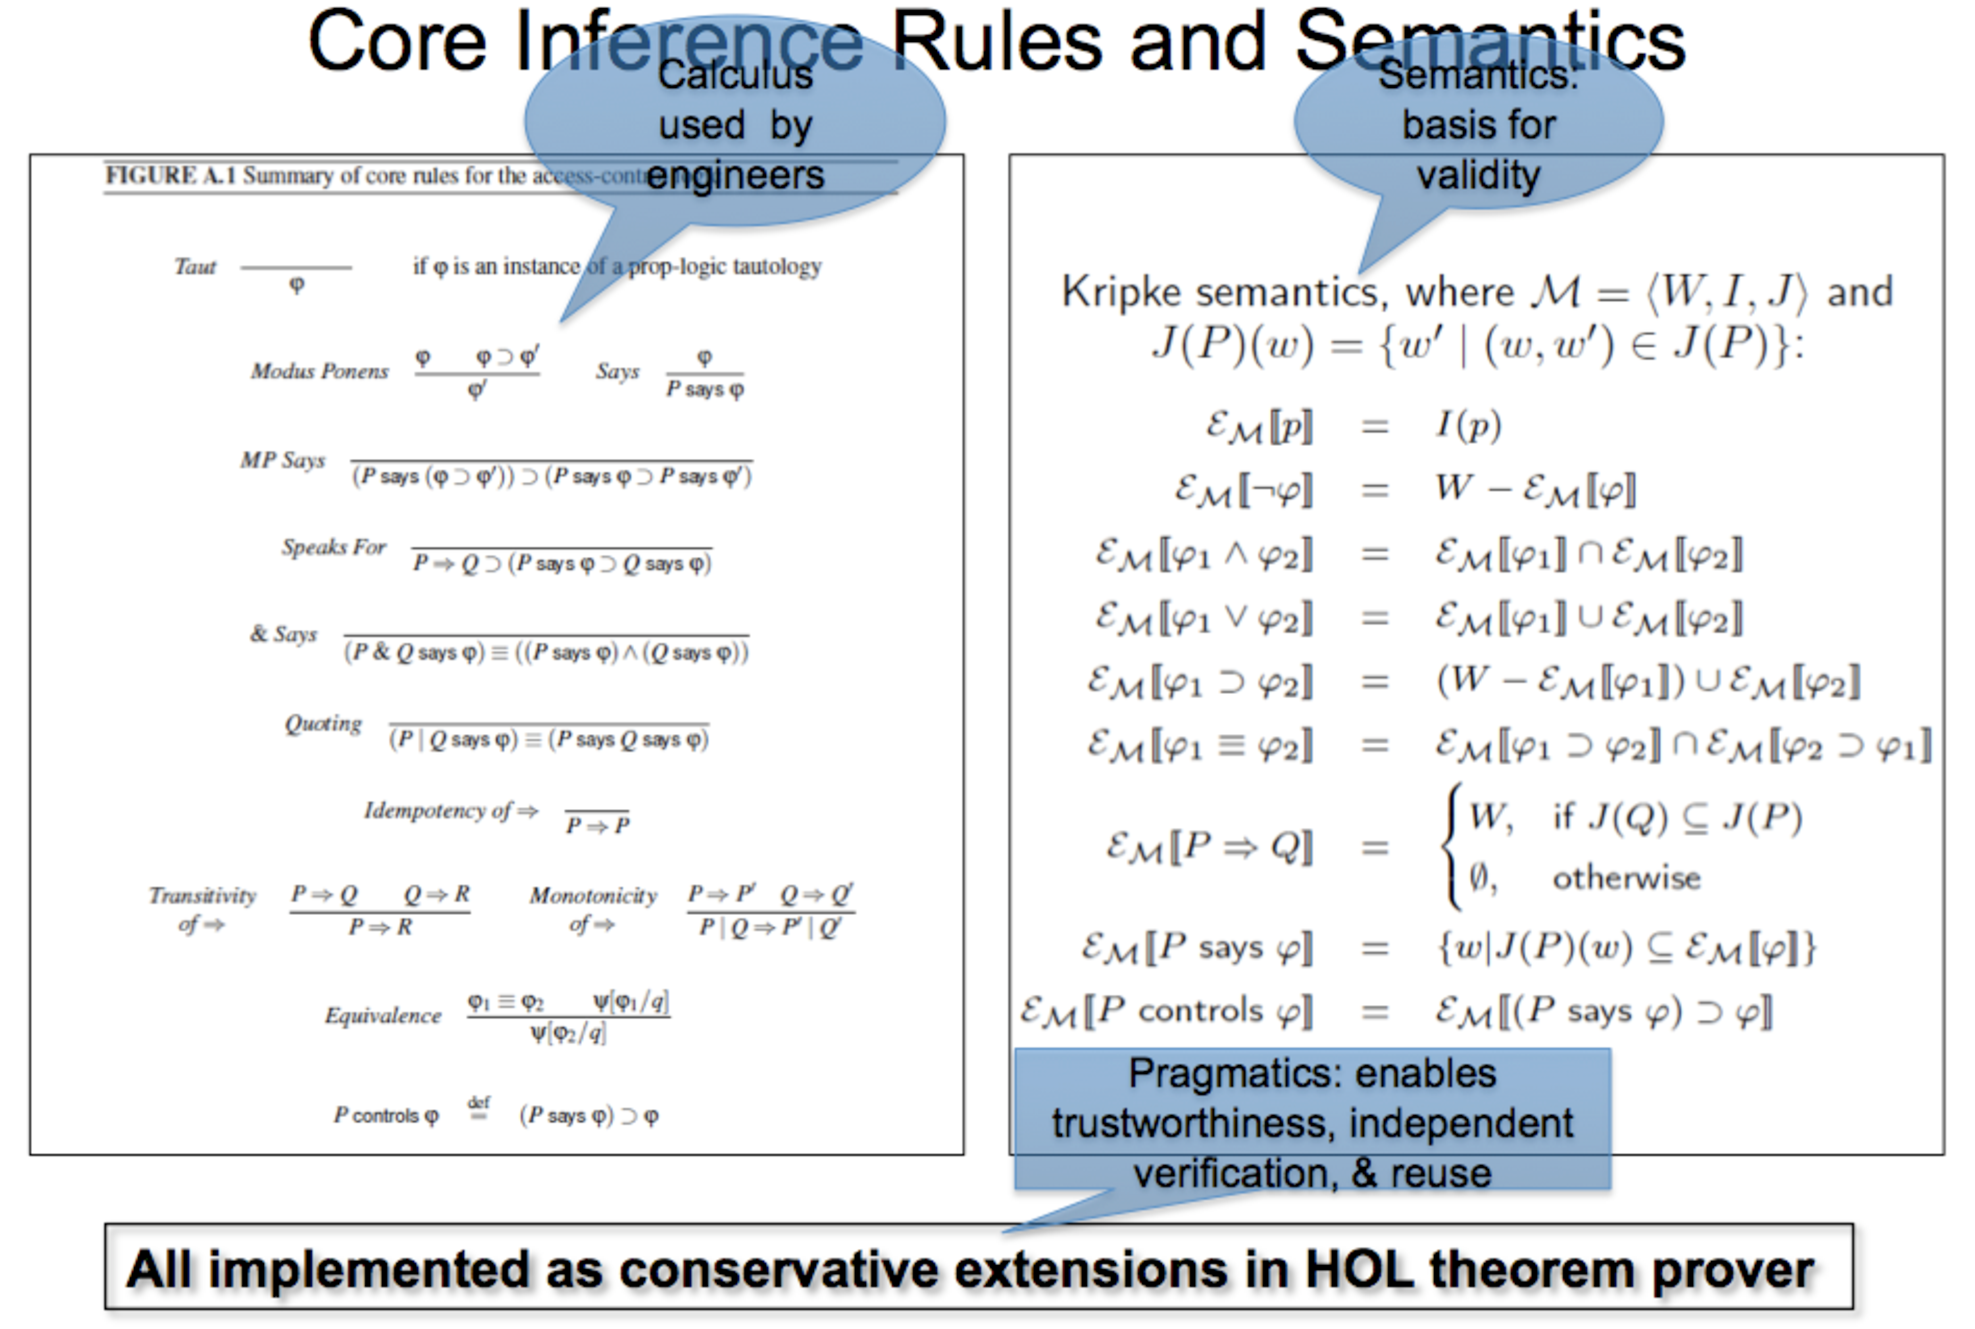
\includegraphics[width=4.0in]{Figures/semantics}
  \end{center}

}

\frame{\frametitle{Example}
  \begin{center}
    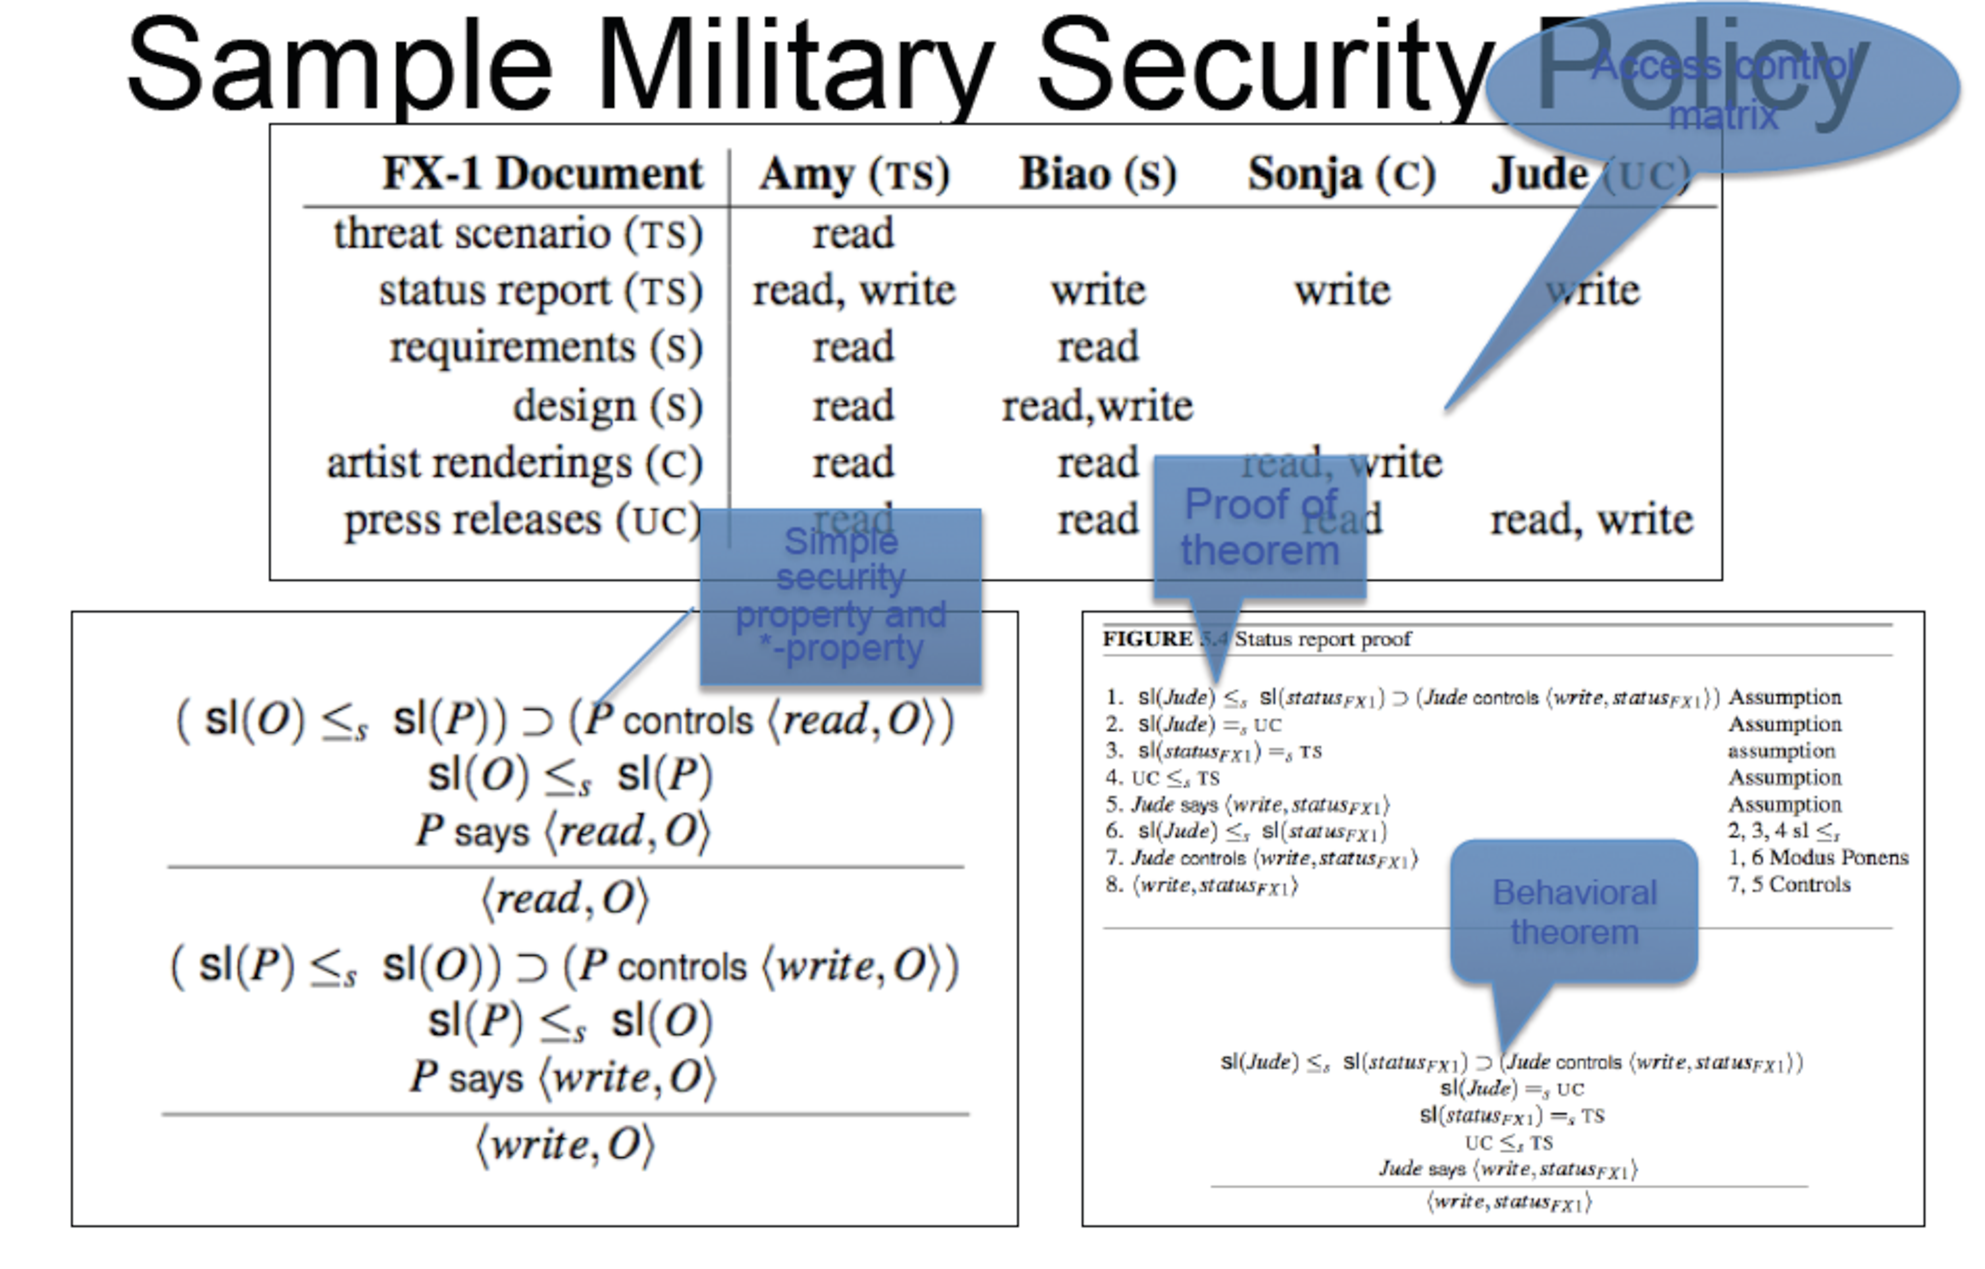
\includegraphics[width=4.0in]{Figures/SecurityPolicy}
  \end{center}
}

\frame{\frametitle{What it looks like in HOL}
  \begin{center}
    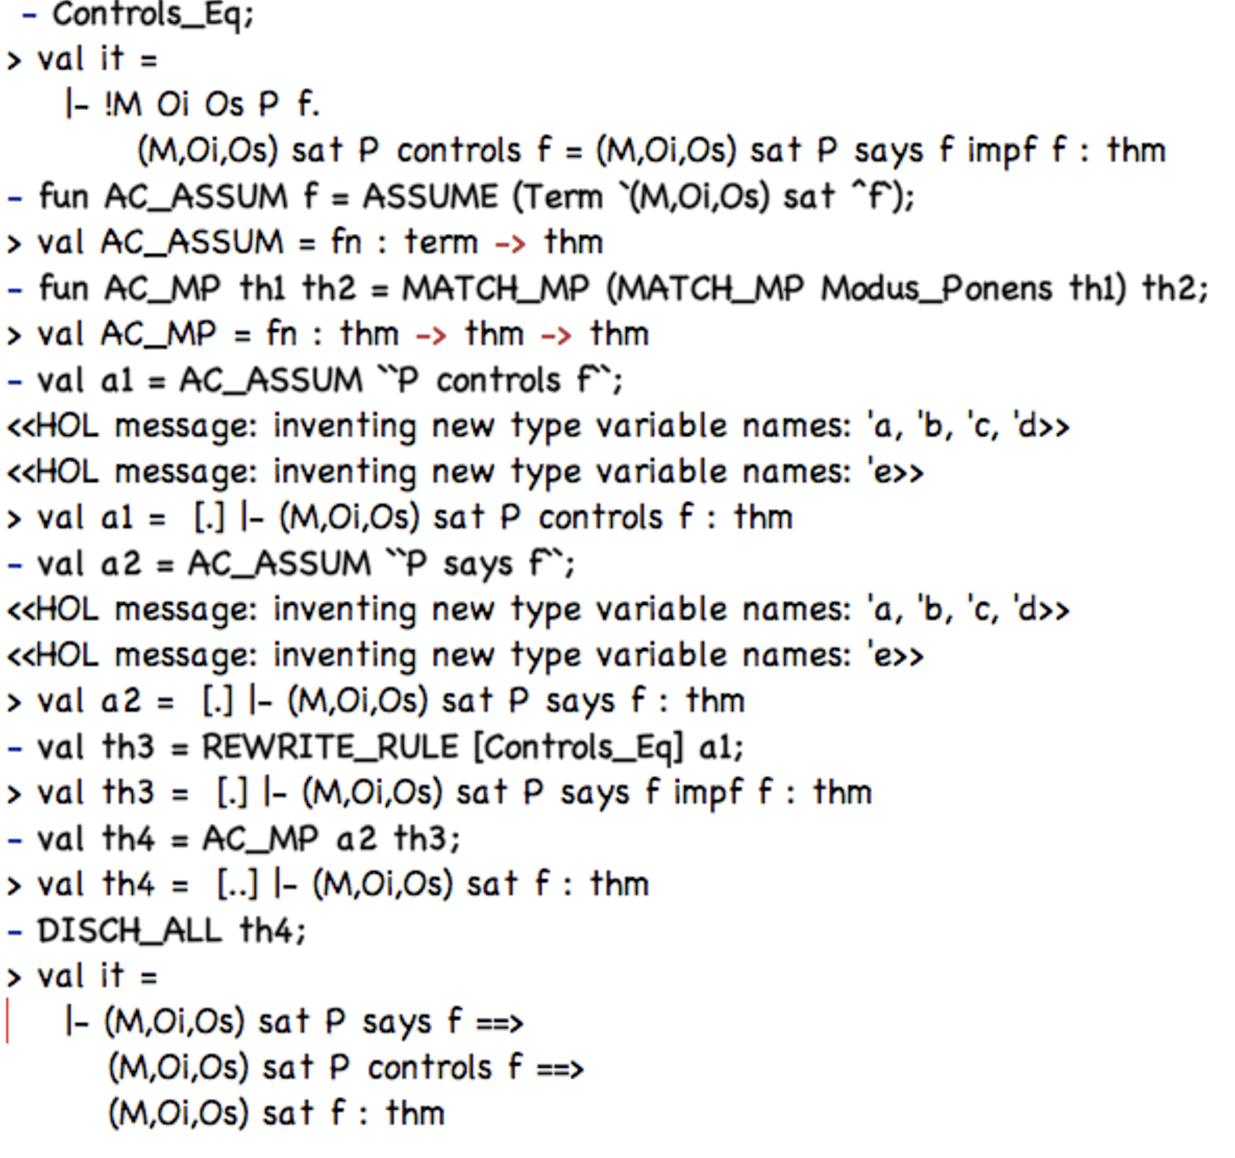
\includegraphics[width=2.7in]{Figures/Proof1}
  \end{center}
}

\end{document}
